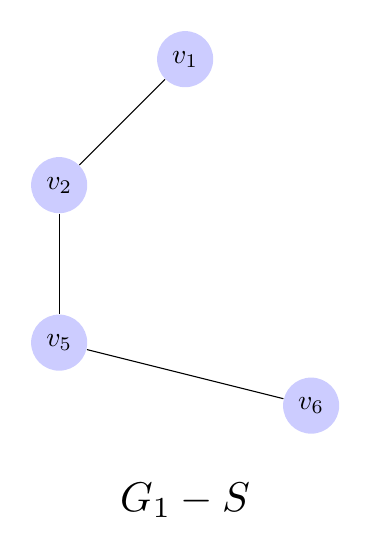
\begin{tikzpicture}
  [scale=.8,auto=left,every node/.style={circle,fill=blue!20}]
\useasboundingbox (0.5,-1.5) rectangle (5.5,6.5);
  \node (n1) at (3,6) {$v_1$};
  \node (n2) at (1,4) {$v_2$};
  \node (n3) at (3,3) [opacity=0]{$v_3$};
  \node (n4) at (5,3) [opacity=0]{$v_4$};
  \node (n5) at (1,1.5) {$v_5$};
  \node (n6) at (5,0.5) {$v_6$};

  \foreach \from/\to in {n1/n2, n2/n5, n5/n6}
    \draw (\from) -- (\to);

   \node[draw=none, fill=none, scale=1.5] at (3,-1) {$G_1-S$};
\end{tikzpicture}
